\documentclass{beamer}
\usefonttheme[onlymath]{serif}

\usepackage[utf8]{inputenc}
\usepackage[T1]{fontenc}
\usepackage{lmodern}
\usepackage[francais]{babel}

% For table
\usepackage{booktabs} % To thicken table lines
\usepackage{multirow}
\usepackage{amsmath}

\usepackage[group-separator={,}]{siunitx}

  %for tikz figure
\usepackage{tikz}
\usetikzlibrary{decorations.pathreplacing}
\usetikzlibrary{fadings}
\usetikzlibrary{positioning} %for lstm
\usetikzlibrary{shapes, backgrounds}
\usetikzlibrary{arrows}
\usetikzlibrary{chains}
\tikzstyle{line} = [draw, -latex']
\usepackage{adjustbox}

\usepackage{pgfplots}
\usepackage{pgfplotstable}

\definecolor{color3}{rgb}{0,0.7,0.3}
\definecolor{color1}{rgb}{0,0.1,0.8}
\definecolor{color2}{rgb}{0.9,0.0,0}

\graphicspath{{img/}}


\mode<presentation> {
	\usetheme{ulaval}
	\setbeamercovered{invisible}
}

\logo{
	
\includegraphics[height=0.65cm, keepaspectratio]{graal.pdf}\hspace{.2cm}\vspace{.85\paperheight}}


\title{Reproductibilité en apprentissage automatique}
%\subtitle[]{}

\author[D. Beauchemin]{David Beauchemin}
\institute[Université Laval]
{
	Département d'informatique et de génie logiciel, \\
	Université Laval\\
	\medskip
	{\emph{david.beauchemin.5@ulaval.ca}}
}
\date{30 octobre 2020}

\AtBeginSection[]
{
	\begin{frame}<beamer>
		\frametitle{Plan}
		\tableofcontents[currentsection, hideallsubsections]
	\end{frame}
}

\begin{document}
	
	
	\begin{frame}[label=titre, plain]
		\titlepage
		\begin{center}
			
\includegraphics[height=1cm]{graal}
			
\includegraphics[height=1cm]{UL_P}
		\end{center}
	\end{frame}

	\begin{frame}{Objectifs de la présentation}
		\begin{itemize}
			\item Sensibiliser sur les enjeux de la reproductibilité.
			\item Inciter l'intégration des solutions permettant une meilleure reproductibilité dans vos solutions d'affaires ou académiques.
		\end{itemize}
	\end{frame}

	\begin{frame}{Mes qualifications}
		\begin{minipage}{0.25\linewidth}
			
\includegraphics[width=\linewidth,keepaspectratio]{david.jpg}
		\end{minipage}
		\hfill
		\begin{minipage}{0.70\linewidth}
		\begin{itemize}
			\item Introduit (informellement) à la recherche reproductible en 2016 (RMarkdown et Git).
			\item Participation à REPROLANG, visant la reproductibilité d'articles scientifiques ayant mené à la publication d'un article en 2020 (où nous abordons les notions présenté ici) \cite{garneau2020robust}.
			\item Membre actif dans le développement de solution d'intégration facilitant la reproductibilité (Poutyne, MLFlow callback).
		\end{itemize}
	  \end{minipage}
	
	\begin{minipage}{0.25\linewidth}
	\small
	\textbf{DAVID BEAUCHEMIN} \\
	Candidat au doctorat \\
	Département d'informatique et de génie logiciel
	\end{minipage}
	\end{frame}
	
	\section{Introduction}
	\begin{frame}{C'est quoi la reproductibilité ?}
		La reproductibilité est le principe qu'on ne peut tirer de conclusions que d'un événement bien décrit, qui est apparu plusieurs fois, provoqué par des \textbf{personnes différentes}.
		
		Toutefois, on utilise souvent ce terme pour spécifiquement désigné la \textbf{réplicabilité}. Soit la réplication (reproduction) des résultats d'un articles dans des environnements pas (toujours) différents \cite{replicationvsreproductiblity, pineau2020improving}.
	\end{frame}

	\begin{frame}{En somme}
		\begin{itemize}
			\item Être capable de répliquer les résultats d'un article/ d'un projet,
			\item à partir du même jeux de données ou un jeux de données différents (mais proche),
			\item en utilisant la procédure d'entrainement de l'article ou en utilisant notre procédure d'entrainement et
			\item en utilisant le code du projet.
		\end{itemize}
	\end{frame}

	\begin{frame}{Pourquoi s'y intéressé?}
		\begin{itemize}
			\item $70$~\% des chercheurs en science on échoué dans leur tentative de reproduire un article d'un autre chercheur,
			\item ~$50$~\% n'on pas réussit à reproduire leur \textbf{propre} expérimentations \cite{baker500ScientistsLift2016}.
		\end{itemize}
	\end{frame}

	\begin{frame}{Pourquoi s'y intéressé?}
		L'informatique ne fais pas exception à cela malgré la simplicité (théorique) de réplication des résultats. Selon une étude, sur 255 articles près de $40$~\% n'était pas réplicable \cite{raff2019step}.
	\end{frame}

	\begin{frame}{Pourquoi s'y intéressé?}
		La réplicabilité du code et d'un article facilite la réutilisation pour d'autres projets de recherche \textbf{et} le transfert vers l'industrie. 
	\end{frame}
	
	\section{Les barrières à la réplicabilité}
%		\begin{frame}
%			\begin{figure}
%				\centering
%				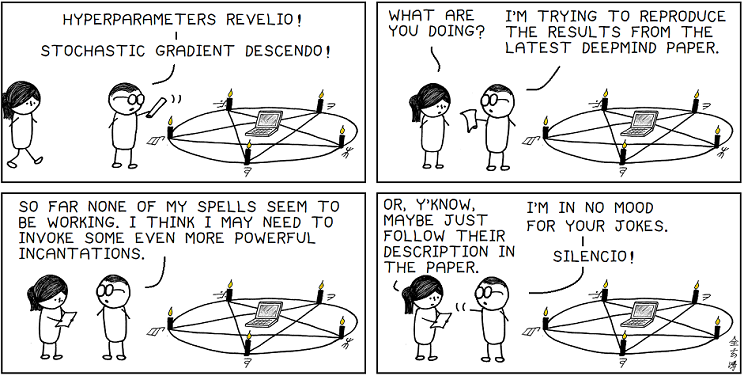
\includegraphics[scale=0.5]{muggle_problems.png}
%				\caption{From Abstruse Goose\footnote{\url{https://abstrusegoose.com/588}}}
%			\end{figure}
%		\end{frame}
	
		\begin{frame}
			\begin{itemize}
				\item Non disponibilité du jeux de données ou version (pas clair) du jeux de données, 
				\item mauvaise spécification ou sous-spécification du modèle ou de la procédure de formation,
				\item manque de disponibilité du code nécessaire pour exécuter les expériences, ou erreurs dans le code,
				\item configuration du modèle déficiente \cite{pineau2020improving}\footnote{Liste sélective de ceux présenté dans l'article.}.
			\end{itemize}
		\end{frame}
	
	\begin{frame}
		\begin{figure}
			\centering
			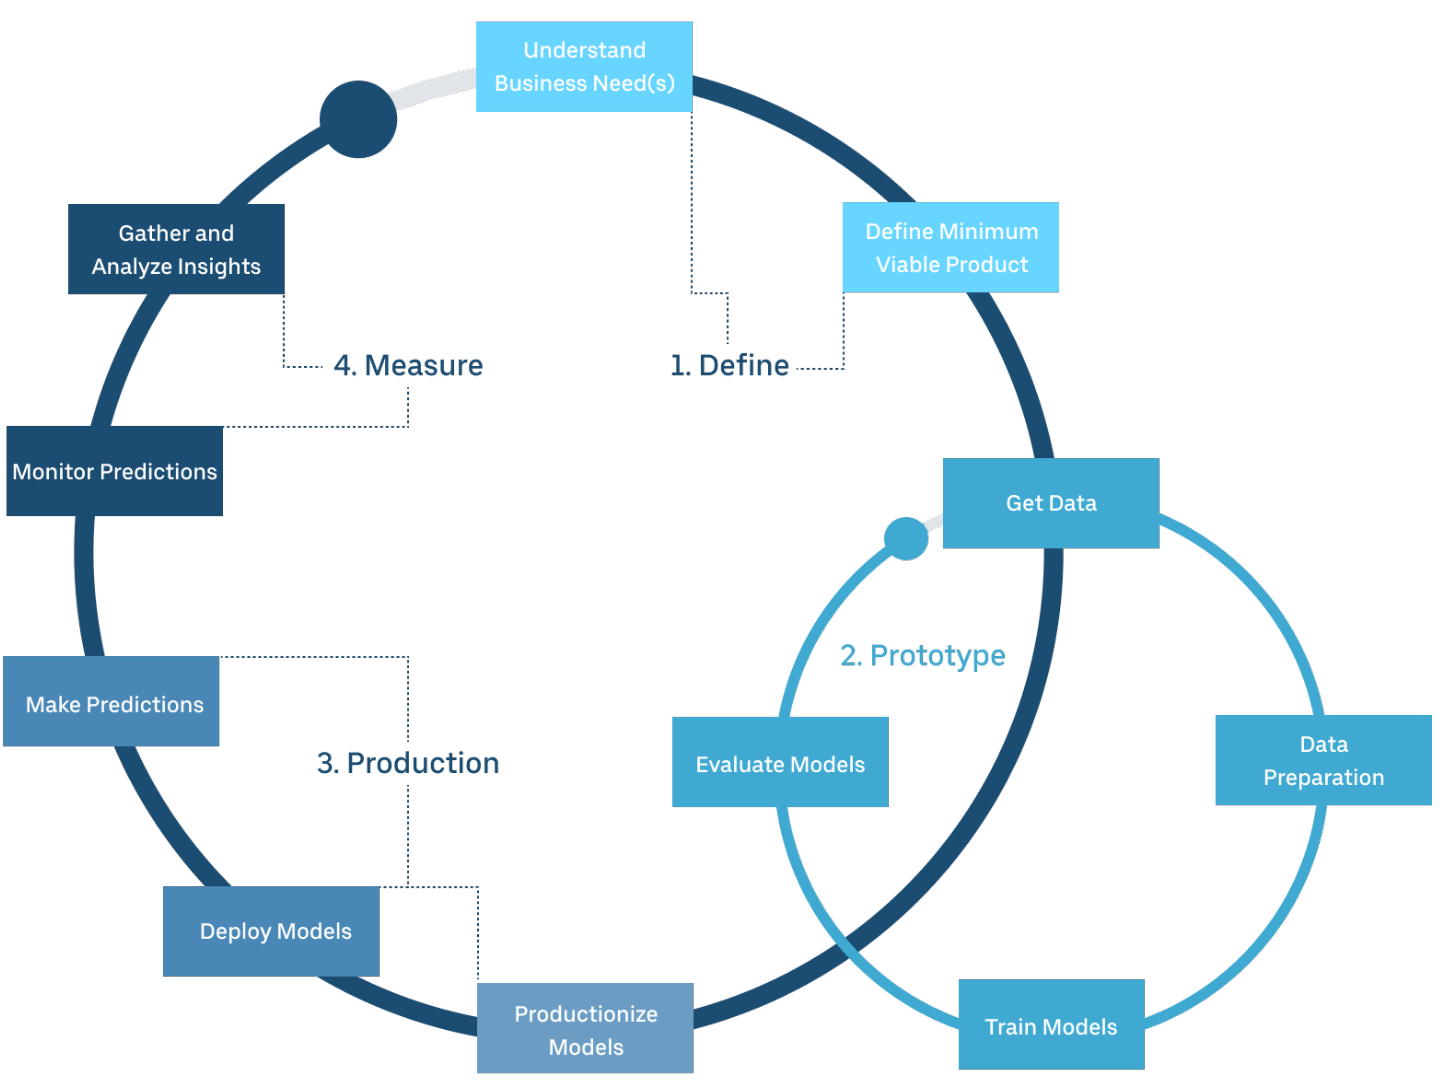
\includegraphics[scale=0.15]{cycle.png}
			\caption{From Uber Engineering\footnote{\url{https://eng.uber.com/scaling-michelangelo/}}}
		\end{figure}
	\end{frame}
	
	\begin{frame}
		\begin{figure}
			\centering
			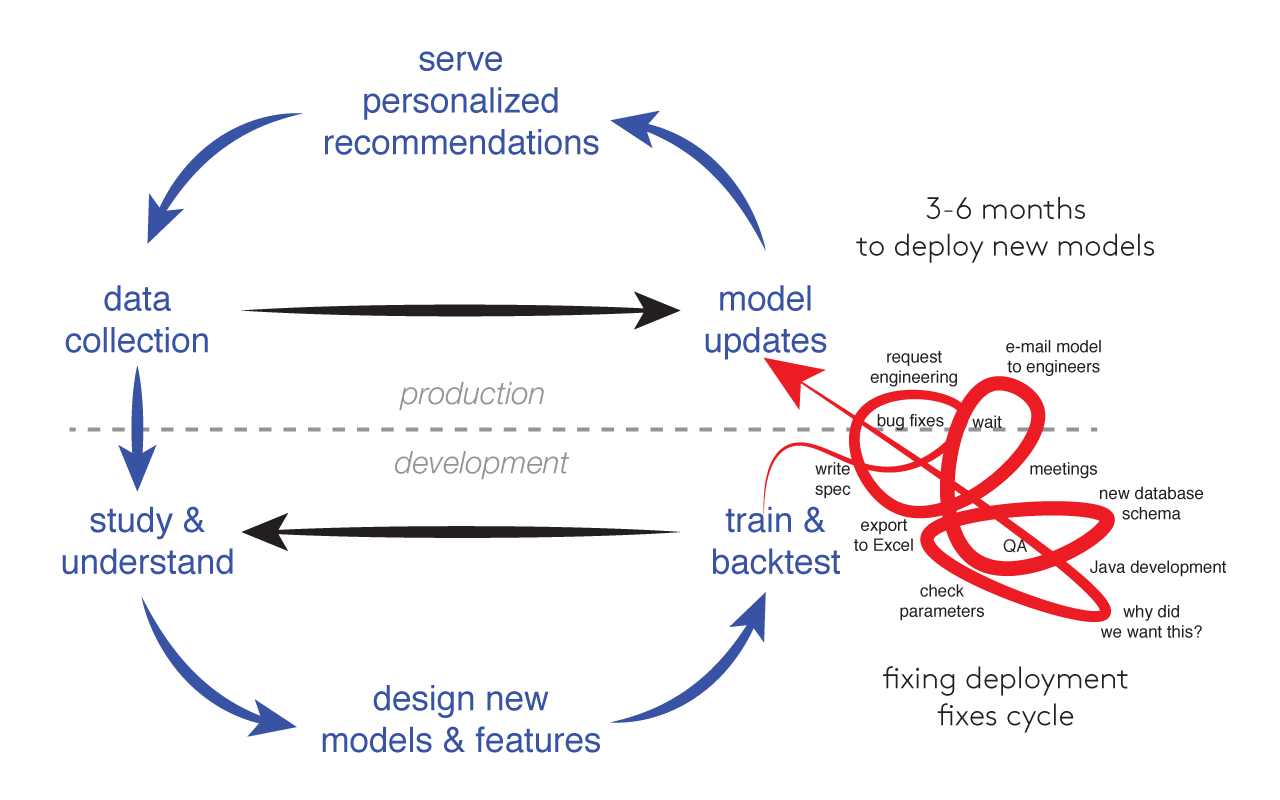
\includegraphics[scale=0.15]{cycle-white.png}
			\caption{The need for Agile machine learning \footnote{\url{https://johann.schleier-smith.com/blog/2015/08/09/need-for-agile-machine-learning.html}}}
		\end{figure}
	\end{frame}
	
	\section{Ok, mais comment?}
	
	\begin{frame}
		\begin{figure}
			\centering
			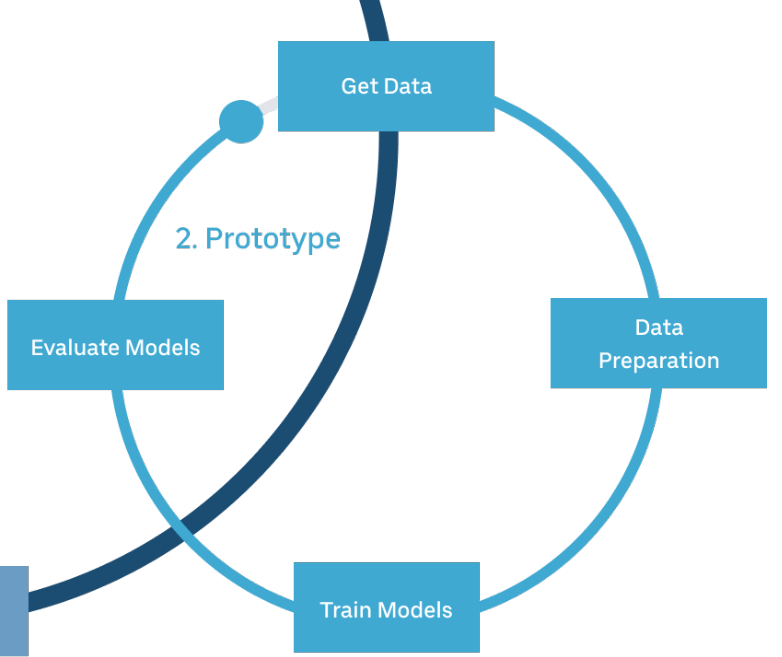
\includegraphics[scale=0.25]{cycle-2.png}
			\caption{From Uber Engineering\footnote{\url{https://eng.uber.com/scaling-michelangelo/}}}
		\end{figure}
	\end{frame}
	\subsection{Données}
	\begin{frame}{Version des données - Étapes de pré-processing}
		\begin{itemize}
			\item Avec qu'elle version des données on travail?
			\item Comment gérer \textbf{facilement} plusieurs version des données?
			\item Comment définir \textbf{facilement} les étapes de pré-processing des données?
		\end{itemize}
		Il nous faut des \textit{data pipelines}, des tuyaux que nous pouvons raccorder \textbf{facilement} à nos modèles pour l'entrainement et la mise en production, par exemple, Data Version Control (DVC)\footnote{https://dvc.org/}.
	\end{frame}

	\subsection{Codes}
	\begin{frame}{Version du code}
		\begin{itemize}
			\item Avec qu'elle version du code on travail?
			\item Comment savoir \textbf{rapidement} qu'elle est la différence d'implémentation entre deux versions du modèles?
			\item Comment gérer \textbf{facilement} les embranchements d'expérimentations?
		\end{itemize}
		Il nous faut un outil nous permettant de visualiser la différence entre des fichiers de code et nous permettant d'avoir plusieurs version du code pouvant exister \textbf{en même temps}, par exemple Git\footnote{https://git-scm.com/}.
	\end{frame}

	\subsection{Développement}
	\begin{frame}{Développement des modèles}
		\begin{itemize}
			\item Ne pas réinventer la roue.
			\item Simplifier l'écriture de code pour développer des modèles.
			\item Qui facilite l'entrainement (GPU, multi-GPU/CPU).
		\end{itemize}
		Il nous faut des outils nous permettant de simplifier le développement de nos modèles, par exemple, Poutyne \cite{poutyne}, PyTorch Lightning \cite{falcon2019pytorch}, Scikit-Learn \cite{sklearn_api}, Gensim \cite{rehurek_lrec} et Allen NLP \cite{Gardner2017AllenNLP}.
	\end{frame}

	\begin{frame}{Entraînement, configuration et résultats}
		\begin{itemize}
			\item Avec qu'elle version du code, du modèle et des données avons-nous fait cet entrainement?
			\item Quels sont les résultats?
			\item Comment visualiser \textbf{rapidement} les résultats et les paramètres de configuration?
		\end{itemize}
		Il nous faut des outils nous permettant de \textit{logger} les paramètres d'entrainement et les résultats, par exemple, MLFlow \cite{Zaharia2018AcceleratingTM} et Sacred \cite{sacred}.
	\end{frame}

	\begin{frame}{Rapport et analyse des résultats}
		\begin{itemize}
			\item Comment créer des tableaux de résultats \textbf{facilement} (pas à la \textit{mitaine})?
			\item Comment s'assurer \textbf{facilement} que les résultats sont à jours?
			\item Comment visualiser \textbf{rapidement} les résultats et les paramètres de configuration?
		\end{itemize}
		Il nous faut des outils nous permettant de créer des tableaux de résultats à même les résultats, soit de diminuer le plus possible le travail manuel, par exemple, Python2latex \footnote{\url{https://github.com/jsleb333/python2latex}} et Markdown \footnote{\url{https://fr.wikipedia.org/wiki/Markdown}}.
	\end{frame}

	\begin{frame}{Dockerisation}
		\begin{itemize}
			\item Comment s'assurer que nos modèles fonctionne sur d'autres environnement?
			\item Comment faciliter la réutilisation de notre code?
		\end{itemize}
		Docker!\footnote{\url{https://www.docker.com/}}
	\end{frame}
	
	%https://gitlab.com/vigou3/webinaire-recherche-reproductible
	
	
	\section{La suite}
	\begin{frame}
		Développer des processus rigoureux (par essai et erreur) et ne pas prendre tout ce qui a été discuter ici comme l'unique solution.
	\end{frame}

	\begin{frame}{Pour aller plus loin}
		\begin{itemize}
			\item Clean code \footnote{\url{https://www.oreilly.com/library/view/clean-code-a/9780136083238/}}
			\item Dagger de projet\footnote{\url{https://github.com/davebulaval/cookiecutter-machine-learning-research}}
		\end{itemize}
	\end{frame}
	
	\begin{frame}[t, allowframebreaks]
		\frametitle{References}
		\bibliographystyle{apalike}
		\bibliography{RAA}
	\end{frame}
	
\end{document}